\documentclass[10pt]{exam}
\usepackage[phy]{template-for-exam}
\usepackage{tikz,graphicx,multicol}

\title{Circular \#1}
\author{Rohrbach}
\date{\today}

\begin{document}
\maketitle

\begin{questions}

\question
  Samuel's father swings him in a circle so that he makes 6 complete rotations in 8 seconds.  Samuel's feet are 1.2 m out from the center of rotation, and his mass is 14 kg.

  \includegraphics[height=4cm]{swinging.jpg}
  %
  \hspace{2in}
  %
  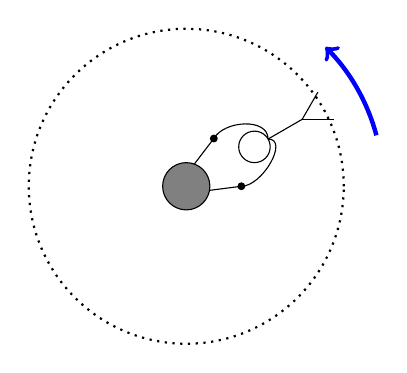
\begin{tikzpicture}

    \filldraw[fill=gray,draw=black] (0,0) 
      circle (.3);
    \draw[dotted,thick] circle (2);

    \begin{scope}
      \draw (30:1) coordinate (head) 
        circle (.2);
      \draw (head) 
        ++(30:.2) coordinate (shoulder)
        -- ++(30:.5) coordinate (waist);
      \draw (waist) -- ++(60:.4);
      \draw (waist) -- ++(0:.4);
      \draw (shoulder) 
        to[out=0,in=0] 
        (0:.7) coordinate (left hand);
      \draw (shoulder) 
        to[out=90,in=60] 
        (60:.7) coordinate(right hand);

    \end{scope}

    \draw (-10:.3) to (left hand);
    \draw (70:.3) to (right hand);
    \fill (right hand) circle (0.05);
    \fill (left hand) circle (0.05);

    \draw[->,ultra thick,blue] (15:2.5) arc (15:45:2.5);


  \end{tikzpicture}
 

 \begin{parts}
   \part 
    What is the tangential speed of Samuel's feet?
    \vs

   \part
    What is Samuel's rotational speed? 
    \vs 

   \part
    What is the force Samuel's father must apply to Samuel to make him move in a circle?
    \vs

 \end{parts}

\question
  You are spinning a ball attached to a rope above your head.  The mass of the ball is 0.1~kg and the radius of the string is 0.6~m. What is the {\bf force of tension} in the rope if the ball has a velocity of 3.1~m/s?
  \vs[2] 

\question
  You are in a car going around a right-hand turn of radius 3.8~m.  The force of friction between your tires and the ground is 79,000~N.  If your car has a mass of 1200~kg, what is the maximum speed you can take through the turn?

  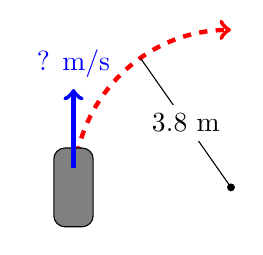
\begin{tikzpicture}
    \draw[dashed, ->, ultra thick, red] 
      (0,0) arc (180:90:2);
    \draw[rounded corners, fill=gray] 
      (-.25,-.5) rectangle ++ (0.5,1);
    \draw[] (2,0) -- ++ (125:2) 
      node[midway, fill=white] {3.8 m};
    \fill (2,0) circle (0.05);
    \draw[->,blue,ultra thick]
      (0,.25) -- ++ (0,1) node[above] {? m/s};
  \end{tikzpicture}
  \vs


\pagebreak

\question
  Explain why your body leans to the left when you make a sharp right turn.
  \vs


\question
  Little Bobby and Janey are both riding a carousel.  Janey is on a pony, which is 5 m from the center of rotation, and Bobby is on a water buffalo, which is 7 m from the center. \label{concept}
  
  \begin{multicols}{2}

    \begin{parts}
      \part
        Which child, if either of them, will have the greater rotational velocity?  Explain.
        \vs

      \part
        Which child, if either of them, will have the greater tangential velocity? Explain.
        \vs
    \end{parts}


    \begin{flushright}
      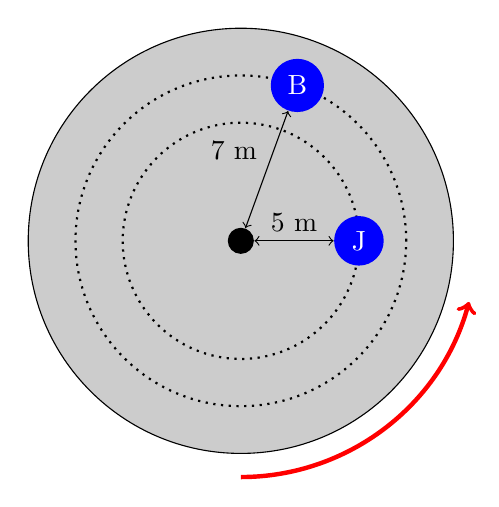
\begin{tikzpicture}[x=3mm,y=3mm]
        \draw[fill=gray!40] (0,0) circle (9);
        \node[circle,minimum size=0.5,fill=black] 
          at (0,0) (center) {};
        \draw[dotted,thick] (0,0) circle (5);
        \draw[dotted,thick] (0,0) circle (7);
        \node[circle,white,fill=blue] at (0:5)
          (Janey) {J};
        \node[circle,white,fill=blue] at (70:7)
          (Bobby) {B};
        \draw[<->] (center) -- (Janey) 
          node[midway,above] {5 m};
        \draw[<->] (center) -- (Bobby) 
          node[midway,above left] {7 m};

        \draw[->,ultra thick,red] (-90:10) arc (-90:-15:10);
      \end{tikzpicture}
    \end{flushright}

  \end{multicols}


\question
  The carousel in the previous problem goes around two times in 90 seconds.  Find the rotational velocity and the tangential velocity of both kids.  (You should have four answers...) \label{math}

  \begin{tabular}{p{2.7in}|p{2.7in}}
    Bobby Tangential & Bobby Rotational \\[10em]\hline
    Janey Tangential & Janey Rotational \\[10em]
  \end{tabular}


\question
  Does your answer for question \ref{math} match what you said in question \ref{concept}?  Explain.
\vspace{0.6in}

\end{questions}

\end{document}